\documentclass[12pt]{article}\usepackage[]{graphicx}\usepackage[]{color}
%% maxwidth is the original width if it is less than linewidth
%% otherwise use linewidth (to make sure the graphics do not exceed the margin)
\makeatletter
\def\maxwidth{ %
  \ifdim\Gin@nat@width>\linewidth
    \linewidth
  \else
    \Gin@nat@width
  \fi
}
\makeatother

\definecolor{fgcolor}{rgb}{0.345, 0.345, 0.345}
\newcommand{\hlnum}[1]{\textcolor[rgb]{0.686,0.059,0.569}{#1}}%
\newcommand{\hlstr}[1]{\textcolor[rgb]{0.192,0.494,0.8}{#1}}%
\newcommand{\hlcom}[1]{\textcolor[rgb]{0.678,0.584,0.686}{\textit{#1}}}%
\newcommand{\hlopt}[1]{\textcolor[rgb]{0,0,0}{#1}}%
\newcommand{\hlstd}[1]{\textcolor[rgb]{0.345,0.345,0.345}{#1}}%
\newcommand{\hlkwa}[1]{\textcolor[rgb]{0.161,0.373,0.58}{\textbf{#1}}}%
\newcommand{\hlkwb}[1]{\textcolor[rgb]{0.69,0.353,0.396}{#1}}%
\newcommand{\hlkwc}[1]{\textcolor[rgb]{0.333,0.667,0.333}{#1}}%
\newcommand{\hlkwd}[1]{\textcolor[rgb]{0.737,0.353,0.396}{\textbf{#1}}}%

\usepackage{framed}
\makeatletter
\newenvironment{kframe}{%
 \def\at@end@of@kframe{}%
 \ifinner\ifhmode%
  \def\at@end@of@kframe{\end{minipage}}%
  \begin{minipage}{\columnwidth}%
 \fi\fi%
 \def\FrameCommand##1{\hskip\@totalleftmargin \hskip-\fboxsep
 \colorbox{shadecolor}{##1}\hskip-\fboxsep
     % There is no \\@totalrightmargin, so:
     \hskip-\linewidth \hskip-\@totalleftmargin \hskip\columnwidth}%
 \MakeFramed {\advance\hsize-\width
   \@totalleftmargin\z@ \linewidth\hsize
   \@setminipage}}%
 {\par\unskip\endMakeFramed%
 \at@end@of@kframe}
\makeatother

\definecolor{shadecolor}{rgb}{.97, .97, .97}
\definecolor{messagecolor}{rgb}{0, 0, 0}
\definecolor{warningcolor}{rgb}{1, 0, 1}
\definecolor{errorcolor}{rgb}{1, 0, 0}
\newenvironment{knitrout}{}{} % an empty environment to be redefined in TeX

\usepackage{alltt}
\usepackage[margin=1in]{geometry}
\usepackage{natbib}
\usepackage{graphicx}
\usepackage{verbatim}
\usepackage{fancyhdr}
\usepackage{amsmath}
\usepackage{lscape}
\usepackage[colorlinks=true,citecolor=black,urlcolor=blue]{hyperref}
\setlength{\headheight}{15pt}

\title{Preliminary Analyses of New York Times Articles\\\large{Version 2}}
\author{Patrick Kraft}
\IfFileExists{upquote.sty}{\usepackage{upquote}}{}
\begin{document}

\maketitle




\section{Description of Dataset}

In order to analyze the content of the NYT articles using the structural topic model approach presented by \citet{roberts2014structural}, I transformed the scraped articles to a reduced dataset where each unique article is included as a \textit{single} observation. Articles that appeared several times in the original raw collection (e.g. most tweeted article for several days) or through different channels (e.g. most tweeted and most viewed) were combined in a single observation. Overall, the reduced dataset contains 5504 \textit{unique} articles for subsequent analyses. Note that the number of articles is slightly lower than in the previous version (5592). I had to scrape the articles again in order to be able to calculate the readability indices (the previous scraping directly pre-processed the articles to omit punctuation etc.) and 88 articles could not be retrieved again in the second scraping. The missing articles were reuters/aponline press releases that were not available on the NYT website anymore.

For each observation, I created a vector of dichotomous variables indicating whether the respective article was included in each of the categories (emailed, facebook, etc.) at least once. Here is a sample of observations from this reduced dataset (article body, keywords, etc. are omitted). These variables represent the matrix of covariates that will be used in order to model differences in topical prevalence in the collection of documents.

\begin{knitrout}
\definecolor{shadecolor}{rgb}{0.969, 0.969, 0.969}\color{fgcolor}\begin{kframe}
\begin{verbatim}
##                title digital_opinion digital_topnews emailed facebook
## 1        My Own Life               1               0       1        1
## 2    The Obama Years               1               0       1        0
## 3  Complete Coverage               0               0       0        0
## 4 Who Loves America?               1               0       1        1
## 5 ISIS Heads to Rome               1               0       1        1
## 6    My Saga, Part 1               0               1       1        1
##   front tweeted viewed digital_bottom
## 1     0       1      1              1
## 2     0       0      1              1
## 3     0       0      1              0
## 4     0       1      1              1
## 5     0       1      1              0
## 6     1       1      1              1
\end{verbatim}
\end{kframe}
\end{knitrout}


\section{Initial Selection Model with 5 Topics}

We decided to focus our analysis on a subset of articles that contain political content. In order to select these articles, I estimated a first structural topic model with 5 topics using the \texttt{stm} package in \texttt{R} \citep[using spectral initialization, see][]{roberts2014structural,roberts2014stm}. In order to make the estimation computationally more tractable, I removed terms from the dictionary that only appeared in 10 articles or less. The following output presents an overview of the extracted topics by displaying words that are highly associated with the respective topic (using highest probability, FREX, Lift, Score, see \citealt{roberts2014stm}).

\begin{knitrout}
\definecolor{shadecolor}{rgb}{0.969, 0.969, 0.969}\color{fgcolor}\begin{kframe}
\begin{verbatim}
## Topic 1 Top Words:
##  	 Highest Prob: said, state, new, republican, presid, will, clinton 
##  	 FREX: republican, clinton, bush, democrat, senat, congress, voter 
##  	 Lift: boehner, rappeport, aipac, asa, burwel, candidaci, caucusgo 
##  	 Score: keyston, republican, obama, clinton, iran, democrat, netanyahu 
## Topic 2 Top Words:
##  	 Highest Prob: one, like, time, said, show, work, new 
##  	 FREX: charact, movi, film, song, novel, book, actor 
##  	 Lift: allegori, bassist, miniseri, penelop, poniewozik, offutt, ballad 
##  	 Score: farmhous, film, music, movi, broadway, book, offutt 
## Topic 3 Top Words:
##  	 Highest Prob: said, state, offici, offic, polic, year, report 
##  	 FREX: islam, polic, besieg, kiir, yemen, salva, etsecretari 
##  	 Lift: assyrian, boko, caliph, debaltsev, haram, jihadi, merga 
##  	 Score: luhansk, islam, polic, yemen, houthi, tikrit, kiir 
## Topic 4 Top Words:
##  	 Highest Prob: new, said, like, citi, york, one, art 
##  	 FREX: chef, runway, wine, museum, restaur, fashion, galleri 
##  	 Lift: anchovi, blanc, brais, breuer, broccoli, caribou, chewi 
##  	 Score: reborn, art, lofi, museum, phillipson, chef, fashion 
## Topic 5 Top Words:
##  	 Highest Prob: said, year, compani, percent, will, one, like 
##  	 FREX: patient, player, fed, investor, basketbal, compani, googl 
##  	 Lift: krzyzewski, antibiot, cholesterol, dekker, epidemiolog, pcs, prey 
##  	 Score: prey, compani, patient, player, coach, game, percent
\end{verbatim}
\end{kframe}
\end{knitrout}

The first topic clearly covers political issues and the US Presidential race. Topic 3 is mostly focused on conflicts, and topic 5 covers a mixture of economic, technology, and sports. Topics 2 and 4, on the other hand, cover cultural themes (movies, museum, fashion, etc.). The heterogeneity in topic 5 indicates that a total number of five topics would be to small to describe the corpus. Nevertheless, this broad categorization is sufficient to select a subset of articles related to political issues for the subsequent analyses. Therefore, I omitted all articles that had the highest probability to belong to topic 2 and 4. Topic 5 was not omitted since it contains articles related to economic issues, which may well be politically relevant. As such, the filtering of political articles can be seen as conservative in the sense that we are more likely to include articles that are not clearly political rather than omitting articles that are. The reduced dataset consists of 3401 articles that were estimated to be most likely to belong to topics 1, 3, or 5.\footnote{It would also be possible to estimate a larger topic model using the entire set of articles and then only focus on topics that are clearly political. The substantive conclusions should not differ with either approach.}


\section{Results for Political/Economic Articles - 10 Topics}

After selecting the subset of articles that focus on political or economic issues, I estimated a second model with 10 topics. The following output again displays the topics along with highly associated words.

\begin{knitrout}
\definecolor{shadecolor}{rgb}{0.969, 0.969, 0.969}\color{fgcolor}\begin{kframe}
\begin{verbatim}
## Topic 1 Top Words:
##  	 Highest Prob: republican, clinton, democrat, senat, presid, new, said 
##  	 FREX: bush, candid, rubio, walker, presidenti, hillari, clinton 
##  	 Lift: chappaqua, nytpolit, rubio, abedin, candidaci, caucusgo, fiorina 
##  	 Score: keyston, clinton, republican, mrs, democrat, bush, presidenti 
## Topic 2 Top Words:
##  	 Highest Prob: said, compani, like, use, servic, new, will 
##  	 FREX: googl, appl, app, internet, technolog, cabl, softwar 
##  	 Lift: byer, ecommerc, gadget, horsepow, jellybeanshap, kleiner, pao 
##  	 Score: prey, googl, compani, app, appl, comcast, technolog 
## Topic 3 Top Words:
##  	 Highest Prob: said, state, offici, islam, presid, countri, govern 
##  	 FREX: iraqi, houthi, milit, ukrain, militia, qaeda, tikrit 
##  	 Lift: abadi, aden, albatati, anbar, fahim, hadi, militiamen 
##  	 Score: luhansk, islam, yemen, houthi, iraqi, tikrit, saudi 
## Topic 4 Top Words:
##  	 Highest Prob: state, said, law, court, feder, rule, case 
##  	 FREX: law, gay, marriag, legal, sex, court, suprem 
##  	 Lift: alito, concur, heterosexu, sotomayor, nondiscrimin, republicandomin, solicitor 
##  	 Score: concur, law, gay, republican, court, marriag, suprem 
## Topic 5 Top Words:
##  	 Highest Prob: said, offic, polic, investig, citi, depart, report 
##  	 FREX: prosecutor, ferguson, polic, manslaught, investig, inmat, guilti 
##  	 Lift: bratton, bureaus, lufthansa, robl, slager, spohr, taser 
##  	 Score: bureaus, polic, ferguson, prosecutor, lubitz, manslaught, inmat 
## Topic 6 Top Words:
##  	 Highest Prob: said, one, peopl, women, school, famili, year 
##  	 FREX: church, cathol, father, women, daughter, girl, campus 
##  	 Lift: turbul, armenian, vatican, devout, priest, pope, bishop 
##  	 Score: turbul, women, armenian, cathol, church, muslim, jew 
## Topic 7 Top Words:
##  	 Highest Prob: iran, state, american, said, agreement, israel, nuclear 
##  	 FREX: nuclear, iran, israel, netanyahu, isra, regim, agreement 
##  	 Lift: arak, bibi, erdbrink, javad, knesset, lausann, natanz 
##  	 Score: knesset, iran, netanyahu, nuclear, israel, iranian, palestinian 
## Topic 8 Top Words:
##  	 Highest Prob: said, health, studi, peopl, school, patient, new 
##  	 FREX: patient, ebola, diseas, cancer, clinic, doctor, studi 
##  	 Lift: dietari, epidemiolog, jama, mutat, placebo, acetaminophen, calori 
##  	 Score: chees, patient, ebola, diseas, cancer, shetreatklein, health 
## Topic 9 Top Words:
##  	 Highest Prob: said, team, game, player, season, play, year 
##  	 FREX: yanke, basketbal, coach, championship, tournament, basebal, season 
##  	 Lift: alderson, catcher, dugout, infield, karlanthoni, layup, ligament 
##  	 Score: katmandu, yanke, coach, basketbal, game, spieth, tournament 
## Topic 10 Top Words:
##  	 Highest Prob: bank, year, compani, said, percent, rate, economi 
##  	 FREX: fed, bank, economi, asset, loan, wage, financi 
##  	 Lift: blackston, buyout, draghi, eurozon, inaccur, suiss, varoufaki 
##  	 Score: inaccur, fed, bank, greec, investor, compani, deutsch
\end{verbatim}
\end{kframe}
\end{knitrout}

The following plot displays the proportions of each individual topic in the overall text body. I added descriptive labels for each topic.

\begin{knitrout}
\definecolor{shadecolor}{rgb}{0.969, 0.969, 0.969}\color{fgcolor}
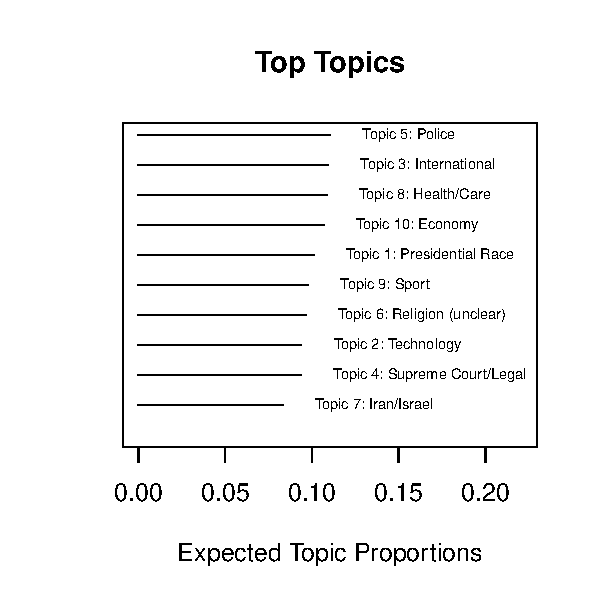
\includegraphics[width=\maxwidth]{figure/unnamed-chunk-5-1} 

\end{knitrout}

Interestingly, the prevalence of topics in the corpus is evenly distributed. However, it should be kept in mind, that each observation in the document matrix can represent multiple instances of an article in the raw collection. The proportions presented here only describe the proportions in unique articles but does not take into account how often each of the articles was included originally (e.g. as most tweeted, or most viewed multiple times). 

We can also directly compare how certain words differentiate between topics. Consider for example topic 1 (presidential race) and topic 3 (international). The following plot displays how certain words are related to each of these topics. The size of the words is proportional to the frequency of occurence in the text, and the position on the x-axis describes whether the word is more related to either of the topics.

\begin{knitrout}
\definecolor{shadecolor}{rgb}{0.969, 0.969, 0.969}\color{fgcolor}
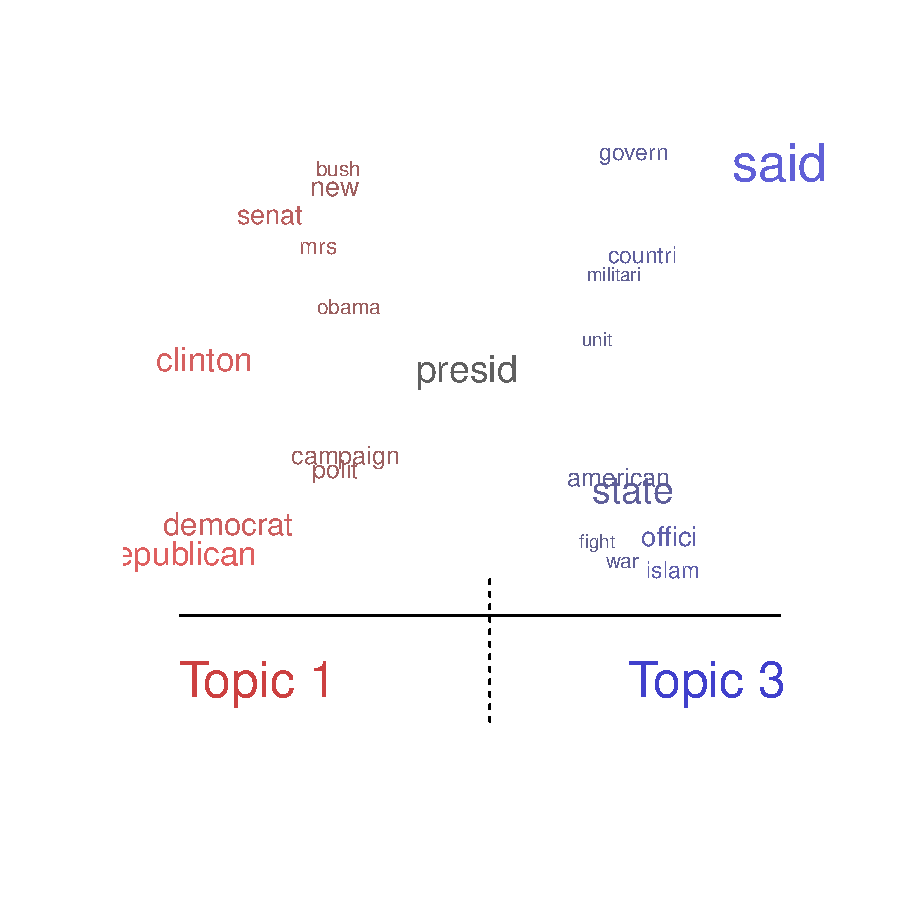
\includegraphics[width=\maxwidth]{figure/unnamed-chunk-6-1} 

\end{knitrout}

In this example, we can see that ``Clinton'' is clearly associated with topic 1 (presidential race), rather than topic 3 (international). The term ``president'' on the other hand, is mentioned frequently in both topics, but cannot be uniquey ascribed to either of the topics. This plausible finding provides some additional face validity for the topic model.


\section{Differences in Topic Proportions between Categories}

As described in \citet{roberts2014structural}, the structural topic model not only extracts topics from a collection of documents but also allows us to directly model the prevalence of topics in specific documents based on a matrix of meta-covariates. While it is also possible to use covariates in order to model differences in words used to describe certain topics, we only focus on differences with regard to \textit{how much} a topic is discussed in specific articles. The following figures display the change in the expected proportion to discuss individual topics for articles that were included in each of the categories or not.

As a first step, we examine topic distributions for content offered by the New York Times through different channels (printed front page vs. digital sections). Looking at the articles that appearead on the printed front page, we can see that the topics ``Technology'' and ``Health/Care'' are less likely to appear. The proportion of articles focusing on both topics is about 5 percentage points lower than in articles that do not appear on the printed front page. Other topics such as ``International'' or ``Police'' are sligthly more likely to be discussed in front page articles. This pattern is even more attenuated when looking at the top news section of the digital edition. Again, ``Technology'' and ``Health/Care'' are less likely to appear (along with ``Sport''). On the other hand, articles in this category were more likely to discuss the presidential race, international affairs, police, as well as relations with Iran and Israel. The bottom section of the digital edition mirrors the topic distribution in the top news section. Here, the proportion of articles related to technology, health, and sport is higher. Lastly, articles in the opinion section were more likely to discuss the Supreme Court and Iran/Israel.


\begin{knitrout}
\definecolor{shadecolor}{rgb}{0.969, 0.969, 0.969}\color{fgcolor}
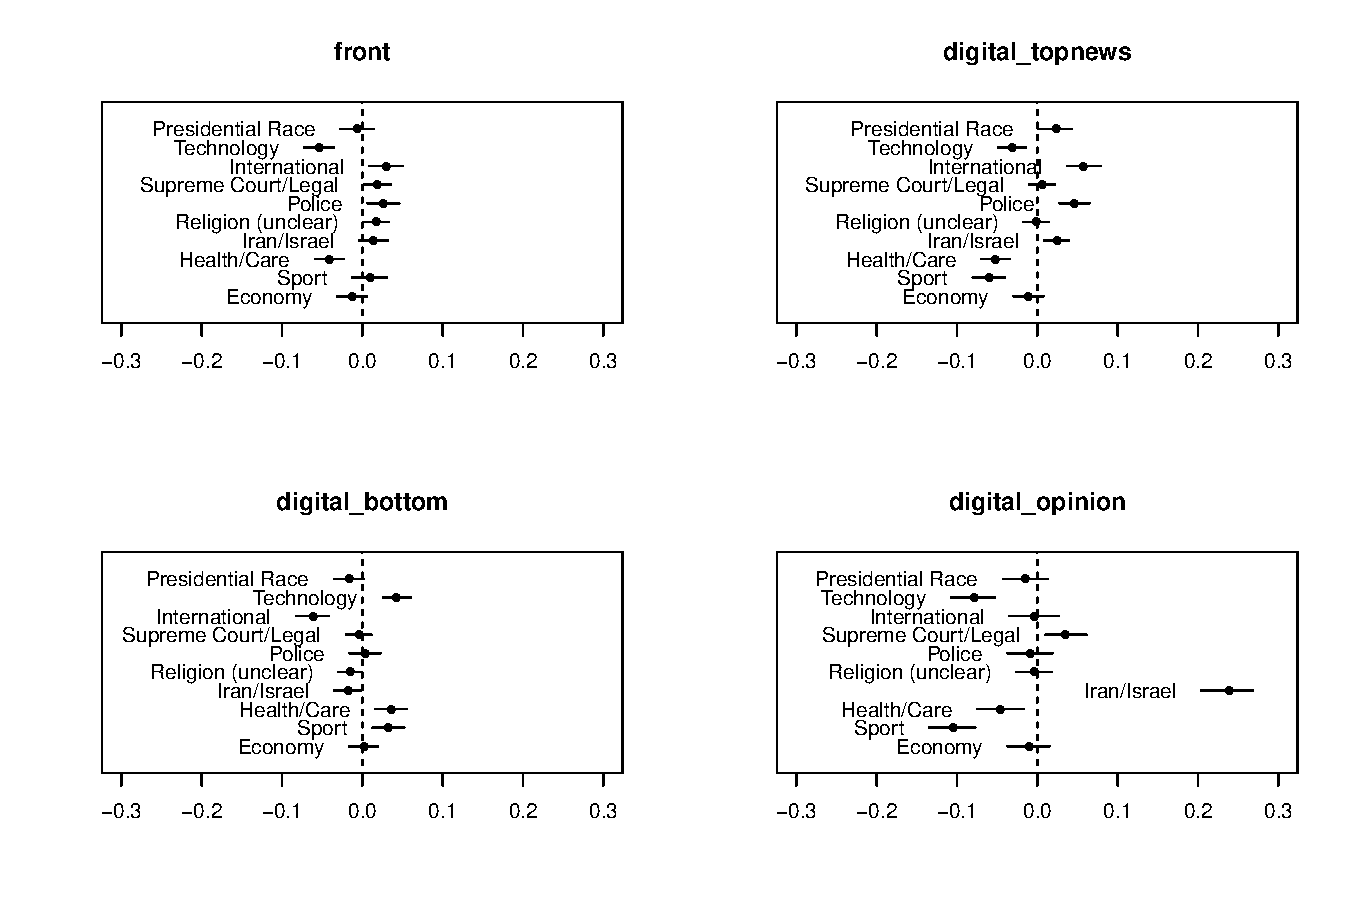
\includegraphics[width=\maxwidth]{figure/unnamed-chunk-7-1} 

\end{knitrout}


Next, we compare topic distributions among articles that were most shared through on different platforms. The figures reveal several interesting patterns. For example, we can see that articles that were most emailed were more likely to belong to the ``Health/Care'' topic but less likely to belong to political topics such as ``Presidential Race'', ``International'', or ``Supreme Court/Legal''. On the other hand, articles that were top shared on facebook were more likely to belong to the topic ``Supreme Court/Legal''. Many articles in this topic discussed same-sex marriage and related Supreme Court decisions. As such, individuals who shared news content on Facebook were more likely to share articles related to marriage equality. Articles shared most on twitter, on the other hand, were more likely to discuss topics of ``Technology''. Overall, the results regarding shared content seem plausible in the context of underlying demographics of the population using each medium.

\begin{knitrout}
\definecolor{shadecolor}{rgb}{0.969, 0.969, 0.969}\color{fgcolor}
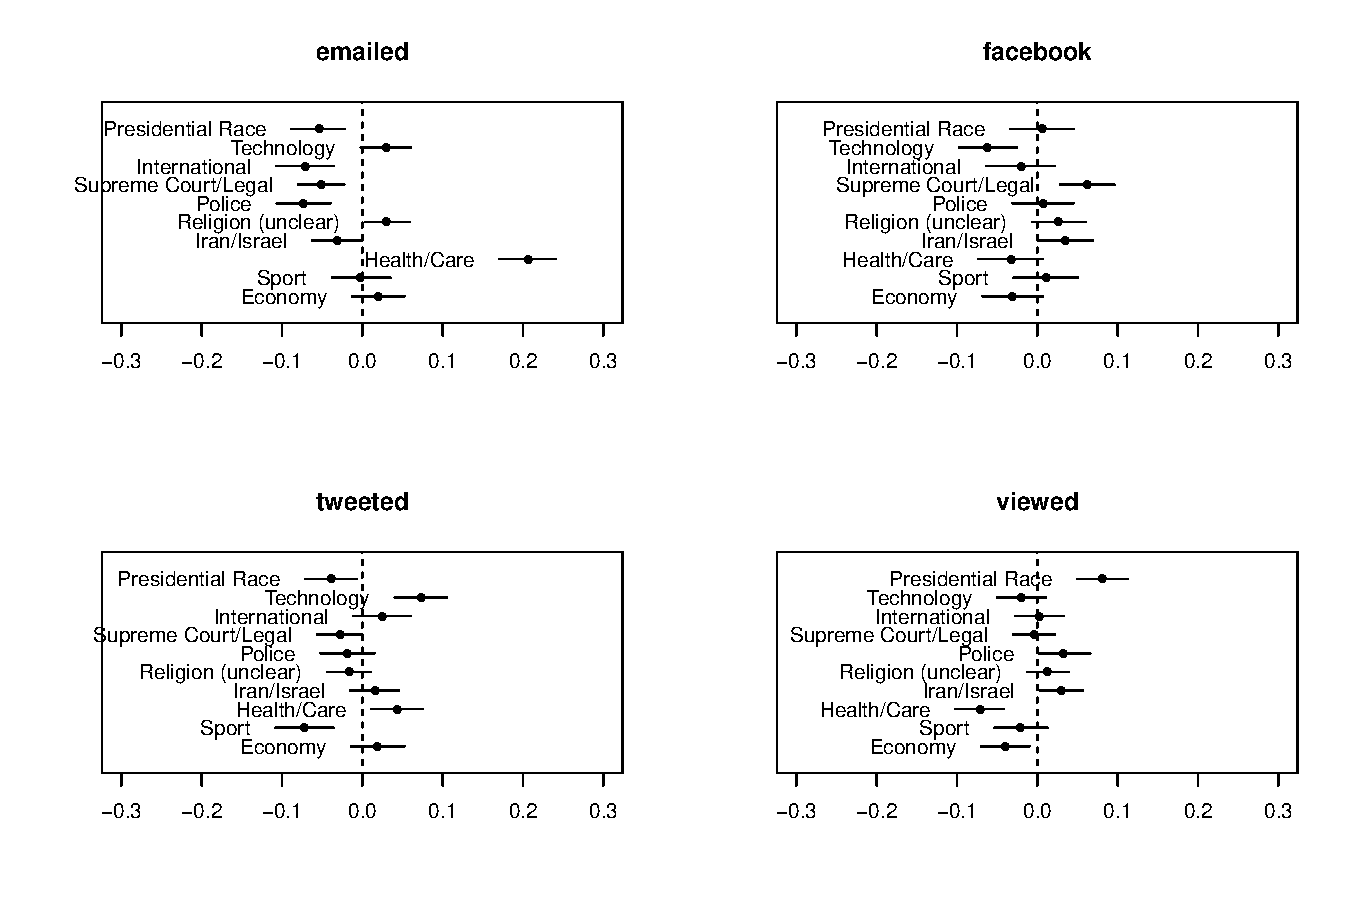
\includegraphics[width=\maxwidth]{figure/unnamed-chunk-8-1} 

\end{knitrout}

How do these patterns translate into views? The last plot (bottom right) of the previous figure displays change in topic proportions for articles that were most viewed. Interestingly, we see that articles in this category were more likely to discuss the presidential race, even though articles in this topic were not more likely to be shared on any platform. Other topics that were more likely in the most-viewed category are ``Police'' and ``Iran/Israel''. Interestingly, while articles about health were more likely to be emailed, they were less likely to be most viewed articles.


\section{Topic Proportions over Time}

We can also examine how the proportion of topics in each of the categories changes over time. Based on the topic model, I matched the estimated topic proportions for each article with the articles' dates of appearance. The following figure displays the aggregate topic proportions for a selection of political topics in each of the article categories from mid February till end of April. Especially the peaks in topic proportions are interesting here. For example, we see that the proportion of articles related to the topic ``Supreme Court/Legal'' in the top news category has a marked increase towards the end of the covered time period. Looking at the articles that were most viewed, we can identify several time points were the presidential race as well as the topic ``Police'' was more salient than other topics.


\begin{knitrout}
\definecolor{shadecolor}{rgb}{0.969, 0.969, 0.969}\color{fgcolor}
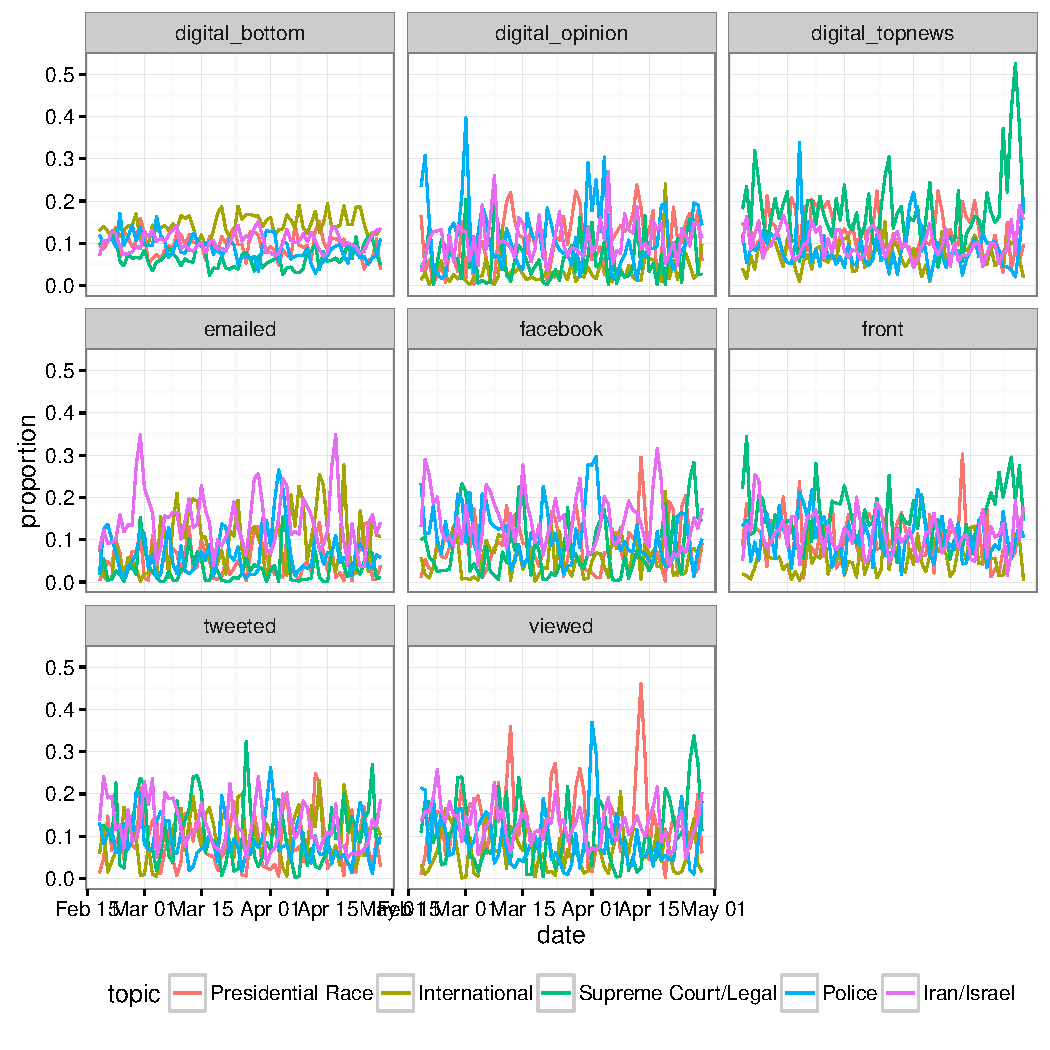
\includegraphics[width=\maxwidth]{figure/unnamed-chunk-9-1} 

\end{knitrout}

\section{Article Readability}

Another interesting question is whether there are structural differences between articles that determine whether they are more likely to be shared/most viewed etc. In order to examine whether the article complexity has any effect, I calculated the Automated Readability Index (ARI) for all articles (there are other readbility indices available, as well). The following figure displays the mean ARI scores for each article category. The ARI is supposed to map onto US school years, so higher numbers indicate higher levels of difficulty. We can observe that articles that were most emailed are on average less complex/difficult to read than articles in any of the remaining categories.

\begin{knitrout}
\definecolor{shadecolor}{rgb}{0.969, 0.969, 0.969}\color{fgcolor}
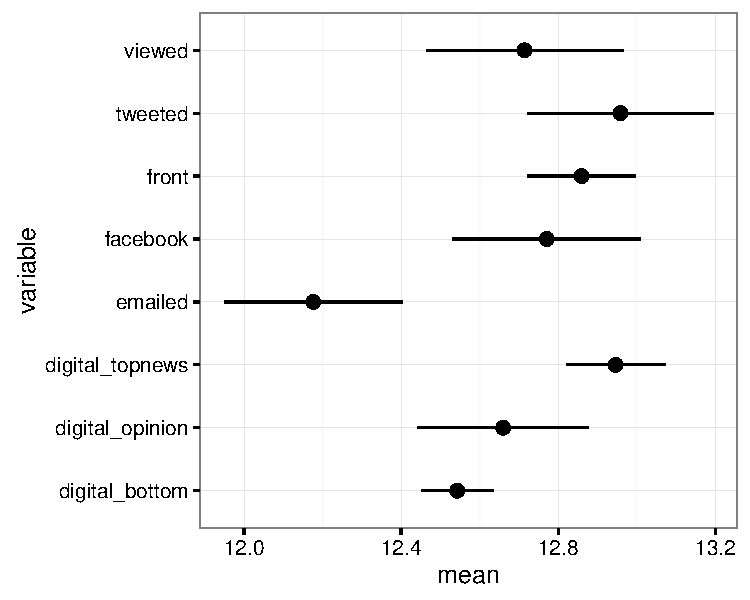
\includegraphics[width=\maxwidth]{figure/unnamed-chunk-10-1} 

\end{knitrout}


\section{What stays in the loop}

As a last step, I started examining the order in which articles appear in each of the categories discussed so far. For example, it could be interesting to see whether articles are first shared and then become most viewed (or vice versa), or whether articles are potentially moved to the top news section after being shared a lot etc. I am not sure yet what the best way is in order to model this since the data structure is quite complex. To get a first impression, I selected all articles that were included in the dataset for mutiple days and calculated the proportion of articles belonging to each category depending on the number of days since the first publication. The following figure displays the results.

\begin{knitrout}
\definecolor{shadecolor}{rgb}{0.969, 0.969, 0.969}\color{fgcolor}
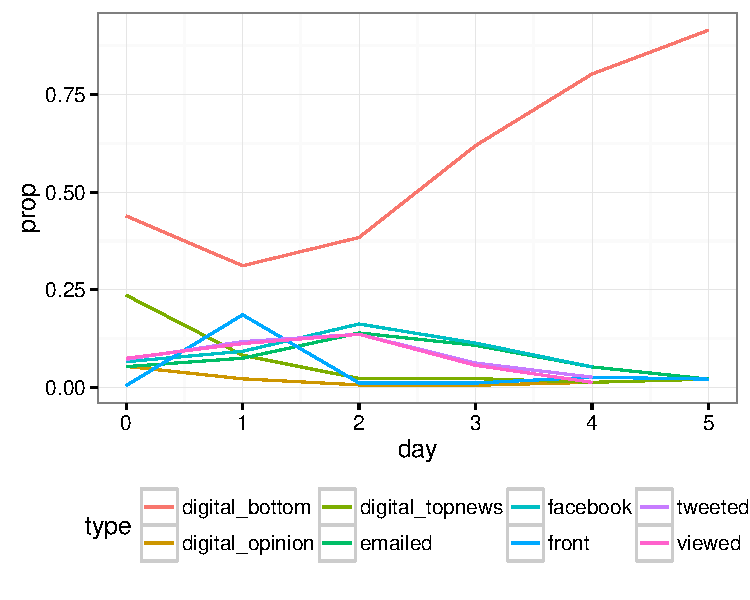
\includegraphics[width=\maxwidth]{figure/unnamed-chunk-11-1} 

\end{knitrout}





\clearpage
\section{Conclusion / Next Steps}
Overall, the structural topic model appears to recover plausible topics from the set of articles analyzed here. Subsequent iterations could investigate results for larger numbers of topics. Furthermore, additional analyses should be conducted in order to check robustness with regard to varying starting values. Other possible subsequent steps include:
\begin{itemize}
  \item investigate influence of other characteristics of articles (e.g. length of article)
  \item link topic model results back to full data, include information about persistence in different categories
  \item set up hazard model, explain how long a topic stays in the cycle
\end{itemize}


\bibliographystyle{/data/Copy/1-src/lit/apsr2006}
\bibliography{/data/Copy/1-src/lit/Literature}
\end{document}

